% !TeX document-id = {a90a2b0a-e08e-44ed-850a-35793bedbf3a}
% !TeX TS-program = xelatex

% !BIB program = biber
\documentclass[handout]{beamer}
%\documentclass[compress]{beamer}
\usepackage[T1]{fontenc}
\usepackage{pifont}
\usetheme[block=fill,subsectionpage=progressbar,sectionpage=progressbar]{metropolis} 


\definecolor{Purple}{HTML}{911146}
\definecolor{Orange}{HTML}{CF4A30}

% Theme colors are derived from these two elements
\setbeamercolor{alerted text}{fg=Orange}

% ... however you can of course override styles of all elements
\setbeamercolor{frametitle}{bg=Purple}


\usepackage{wasysym}
\usepackage{etoolbox}
\usepackage[utf8]{inputenc}

\usepackage{threeparttable}
\usepackage{subcaption}

\usepackage{tikz-qtree}
\setbeamercovered{still covered={\opaqueness<1->{5}},again covered={\opaqueness<1->{100}}}


\usepackage{listings}

\lstset{
	basicstyle=\scriptsize\ttfamily,
	columns=flexible,
	breaklines=true,
	numbers=left,
	%stepsize=1,
	numberstyle=\tiny,
	backgroundcolor=\color[rgb]{0.85,0.90,1}
}



\lstnewenvironment{lstlistingoutput}{\lstset{basicstyle=\footnotesize\ttfamily,
		columns=flexible,
		breaklines=true,
		numbers=left,
		%stepsize=1,
		numberstyle=\tiny,
		backgroundcolor=\color[rgb]{.7,.7,.7}}}{}


\lstnewenvironment{lstlistingoutputtiny}{\lstset{basicstyle=\tiny\ttfamily,
		columns=flexible,
		breaklines=true,
		numbers=left,
		%stepsize=1,
		numberstyle=\tiny,
		backgroundcolor=\color[rgb]{.7,.7,.7}}}{}


\usepackage[american]{babel}
\usepackage{csquotes}
\usepackage[style=apa, backend = biber]{biblatex}
\DeclareLanguageMapping{american}{american-UoN}
\addbibresource{../literature.bib}
\renewcommand*{\bibfont}{\tiny}

\usepackage{tikz}
\usetikzlibrary{shapes,arrows,matrix}
\usepackage{multicol}

\usepackage{subcaption}

\usepackage{booktabs}
\usepackage{graphicx}

\graphicspath{{../pictures/}}

\makeatletter
\setbeamertemplate{headline}{%
	\begin{beamercolorbox}[colsep=1.5pt]{upper separation line head}
	\end{beamercolorbox}
	\begin{beamercolorbox}{section in head/foot}
		\vskip2pt\insertnavigation{\paperwidth}\vskip2pt
	\end{beamercolorbox}%
	\begin{beamercolorbox}[colsep=1.5pt]{lower separation line head}
	\end{beamercolorbox}
}
\makeatother



\setbeamercolor{section in head/foot}{fg=normal text.bg, bg=structure.fg}



\newcommand{\question}[1]{
	\begin{frame}[plain]
		\begin{columns}
			\column{.3\textwidth}
			\makebox[\columnwidth]{
				
\includegraphics[width=\columnwidth,height=\paperheight,keepaspectratio]{../pictures/mannetje.png}}
			\column{.7\textwidth}
			\large
			\textcolor{orange}{\textbf{\emph{#1}}}
		\end{columns}
\end{frame}}

\newcommand{\instruction}[1]{\emph{\textcolor{gray}{[#1]}}}


\title[Computational Communication Science 2]{\textbf{Computational Communication Science 2} \\Week 1 - Lecture\\ »Introduction«}
\author[Marthe Möller, Anne Kroon]{Marthe Möller \\ Anne Kroon \\ ~ \\ \footnotesize{A.M.Moller@uva.nl, @MartheMoller \\a.c.kroon@uva.nl, @annekroon} \\}
\date{April, 2022}
\institute[Digital Society Minor, University of Amsterdam]{Digital Society Minor, University of Amsterdam}


\begin{document}
	
	\begin{frame}{}
		\titlepage
	\end{frame}
	
	\begin{frame}{Today}
		\tableofcontents
	\end{frame}

\begin{frame} 
	All course materials can be found at\ldots \\
	~~~~~~~~\url{https://github.com/annekroon/CCS-2}
\end{frame}

\section{Introducing\ldots the people}


\begin{frame}{Introducing\ldots \huge{Marthe}} 
	
	\begin{columns}
		\column{.3\textwidth}
		\makebox[\columnwidth]{
			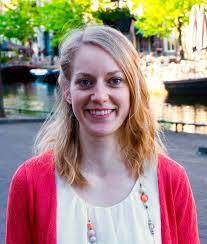
\includegraphics[width=\columnwidth,height=\paperheight,keepaspectratio]{../pictures/marthe.jpg}}
		\column{.7\textwidth}
		dr. A. Marthe Möller \\
		Assistant Professor Entertainment Communication
		\begin{itemize}
			\item Studying entertainment experiences in the digital space using:
			\begin{itemize}
				\item Computational methods (e.g., ACA of user comments)
				\item Experimental methods
			\end{itemize}
		\end{itemize}
		@marthemoller \textbar A.M.Moller@uva.nl \textbar \url{https://www.uva.nl/profiel/m/o/a.m.moller/a.m.moller.html} 
	\end{columns}
\end{frame}

\begin{frame}{Introducing\ldots \huge{Anne}} 
	\begin{columns}[] \column{.3\textwidth} \makebox[\columnwidth]{ 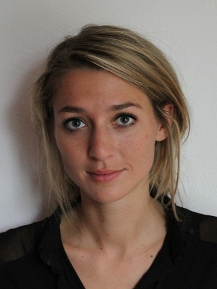
\includegraphics[width=\columnwidth,height=\paperheight,keepaspectratio]{../pictures/anne.jpg}} \column{.7\textwidth} dr. Anne Kroon \\ 
		Assistant Professor Corporate Communication
		\begin{itemize} 
			%\item Studied Journalism and Communication,  2006 - 2013
			%\item PhD candidate corporate communication at ASCoR (University of Amsterdam), 2014 - 2017
			\item Research focus on biased AI in recruitment, and media bias regarding minorities
			\item Text analysis using automated approaches, word embeddings
		\end{itemize} @annekroon \textbar a.c.kroon@uva.nl  \textbar \url{http://www.uva.nl/profiel/k/r/a.c.kroon/a.c.kroon.html} 
	\end{columns} 
\end{frame}


\begin{frame}{Introducing\ldots \huge{You}}
	{\huge{You}}
	\small{}
	\begin{columns}
		\column{.3\textwidth}
		\makebox[\columnwidth]{
			
\includegraphics[width=\columnwidth,height=\paperheight,keepaspectratio]{../pictures/mannetje.png}}
		\column{.7\textwidth}
		Your name?\\
		Your background?\\
		Your reason for taking this course?\\
		Do you have a dataset you are working on?
	\end{columns}
\end{frame}


\section{Introducing\ldots the course}


\begin{frame}{About CCS-2} 

What is CCS-2?
	\begin{itemize}
		\item Next step after CCS-1 %we assume you know the basics!
		\item How to use what you learned in CCS-1 for research?
		\begin{itemize}
			\item Learn computational techniques (e.g. data vectorization, machine learning)
			\item Learn how to use these techniques for research (e.g., content analysis)
		\end{itemize}
		\item By the end of the course, you'll be prepared to do computational research in the Research Project
	\end{itemize}
	
\end{frame}


\begin{frame}{About CCS-2}
	
	\begin{center}
		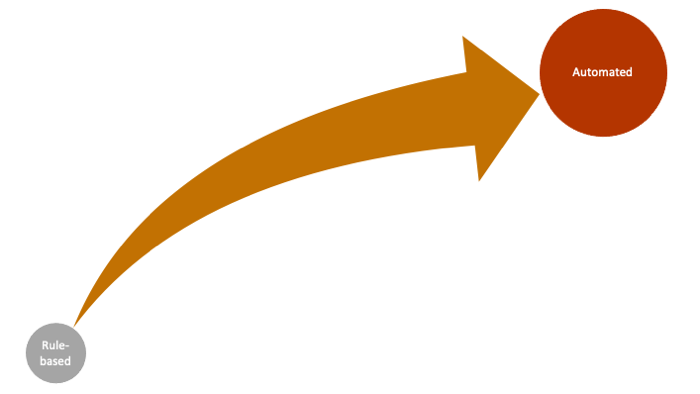
\includegraphics[width=\linewidth,height=\textheight,keepaspectratio]{../pictures/Roadmap.png} 
	\end{center}
	
\end{frame}


\begin{frame}{About CCS-2}
	
	\begin{center}
		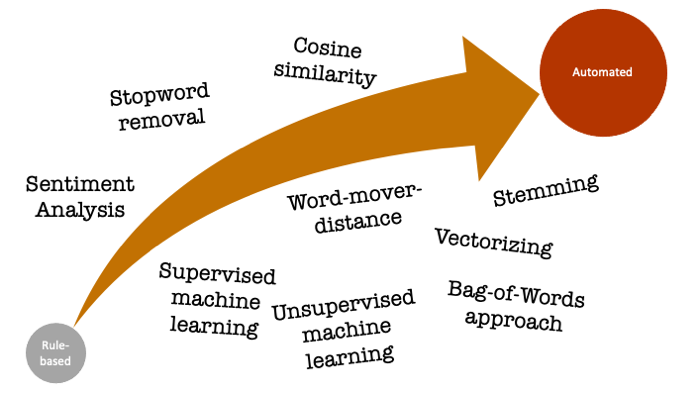
\includegraphics[width=\linewidth,height=\textheight,keepaspectratio]{../pictures/Roadmap_terms.png} 
	\end{center}
	
\end{frame}


\begin{frame}{About CCS-2} 

What will we do in this course?	
	\begin{itemize}
		\item We discuss techniques in the lectures
		\item We practice with techniques in the tutorials
		\item Graded assignments to master the techniques:
		\begin{itemize}
			\item Regular multiple choice questions (\(20\%\)) about readings that use the techniques we discuss
			\item Coding challenge (group assignment): Get more experienced with the techniques and build a recommender system
			\begin{itemize}
				\item Report (\(20\%\))
				\item Presentation (\(10\%\))
			\end{itemize}
			\item Take-home exam (\(50\%\)) at the end of the course so you can show off what you learned
		\end{itemize}
		\item We provide structure through the meetings and assignments, you do the (home-)work
	\end{itemize}
	
\end{frame}



\begin{frame}{About CCS-2} 
	
	How to stay informed and where to find all the materials? Regularly check:	
	\begin{itemize}
		\item The course Canvas page
		\item Your email
		\item The course Github page
	\end{itemize}

	In addition, make sure that you read the course manual so that you know all the ins and outs of this course!

\end{frame}


\begin{frame}{About CCS-2} 
	
	How to contact Anne and Marthe?	
	
	\textcolor{red}{We kunnen hier eventueel iets over zeggen: mogen ze mailen, zijn er spreekuren etc.?}
	
\end{frame}

\begin{frame}{Ready? Set? Go!} 
	
	Without further ado\dots
	
	\dots let's get started!
	
\end{frame}



\section{Text as Data}


\begin{frame}{Text as Data}
	
CCS-1: You learned how to...
	\begin{itemize}
	\item Work with Python, for example, you:
	\begin{itemize}
		\item Store text in json-files, csv-files etc.
		\item Work with texts in Python
	\end{itemize}
\end{itemize}
	
\end{frame}

\begin{frame}{Text as Data}
	
	Studying text can teach us a lot about human behavior: \\~
	
	What topics do people discuss on online cancer-related platforms? \\
	\begin{tiny}
		(\cite{sanders_different_2020}) \\
	\end{tiny}

	To what extent does content differ between online and print news? \\
	\begin{tiny}
	(\cite{burggraaff_through_2020}) \\
	\end{tiny}

	What topics do people discuss in their movie reviews? \\
	\begin{tiny}
	(\cite{schneider_what_2020}) \\
	\end{tiny}	

% Within communication science, text is often the subject of study
	
\end{frame}


\begin{frame}{Text as Data}
	
	Studying text can give us information we can use to answer broader questions: \\~
	
	Analyze textual information about movies from IMDB to learn about the representation of women in movies \\
	\begin{tiny}
	(\cite{poma-murialdo_gender_2019}) \\
	\end{tiny}

	Automatically distinguish between reliable and unreliable online information about vaccines by investigating what characterizes reliable and unreliable texts \\
	\begin{tiny}
	(\cite{meppelink_reliable_2021}) \\
	\end{tiny}	
	
	% Within communication science, text is often the subject of study
	
\end{frame}


\begin{frame}{Text as Data}
	
	We can use data about text in combination with other methods: \\~
	
	Combining data about media content and survey data to investigate how media coverage affects citizens' trust in the EU \\
	\begin{tiny}
		(\cite{brosius_trust_2019}) \\
	\end{tiny}
	
	
	% Within communication science, text is often the subject of study
	
\end{frame}


\section{Analyzing songtexts}

\begin{frame}[fragile]{Analyzing songtexts}
	
	What did people sing about in traditional songs? 
	\begin{lstlisting}

		texts = ["Of all the money that e'er I had, I spent it in good company", "Down by the Sally Gardens, my lover and I did meet", "Speed, bonny boat, like a bird on the wing"]

	\end{lstlisting}
	
	\begin{lstlistingoutput}
		[('really', 3), ('I', 2), ('love', 1)]
		[('I', 1), ('hate', 1), ('him', 1)]
	\end{lstlistingoutput}
\end{frame}


%hier verder en met dit voorbeeld deze dingen bespreken: Working with strings, Text cleaning = stopword removal, punctioation and noise removal, and regexp



\end{document}